Como o exercício fornece os lados do triângulo, é possível calcular sua área
total pela fórmula de Heron:

Área = $\sqrt{p(p-L1)(p-L2)(p-L3)}$ , sendo $p$ o semiperímetro:
$p = \displaystyle\frac{L1+L2+L3}{2}$.

Dessa forma:

\begin{center}
    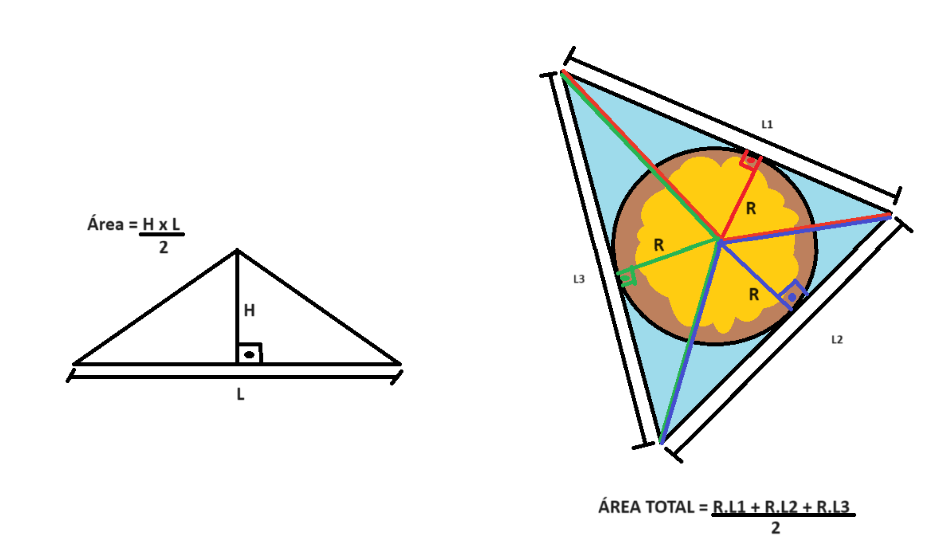
\includegraphics[scale=0.4]{vasilhaerrada/editorial.png}
\end{center}

Isolando $R$, tem-se que $R=\displaystyle\frac{\text{Área total}}{P}$.

Complexidade: $O(1)$.
